En la actualidad nos enfrentamos a una gran variedad de desastres, tanto naturales como provocados por el ser humano: desde terremotos, inundaciones y huracanes, hasta actos de terrorismo. En estas situaciones entran en acción diversos equipos de respuesta como pueden ser policías, bomberos o para-médicos entre otros, que trabajan conjuntamente para preservar vidas, proteger infraestructuras y evacuar a las víctimas. Por fortuna, la tecnología también está jugando un papel importante, apoyando algunas tareas que los seres humanos y los perros no pueden hacer por sí sólos.

Tal vez, la primera intervención robótica en una tarea de inspección y rescate tras un desastre documentada, fue la llevada a cabo por los robots de William “Red” Whittaker en el Field Robotics Center (Carnegie Mellon University) en el año 1979, para inspeccionar el estado del reactor de la central nuclear de Three Mile Island tras el accidente sufrido.

Posteriormente se han documentado diferentes intervenciones robóticas de alta relevancia como pueden ser los utilizados tras el accidente nuclear de la central de Fukushima (2011) y tras los terremotos de Haiti (2010) o Nepal (2015).

\begin{figure}[H]
    \centering
    \begin{subfigure}[c]{0.45\textwidth}
        \centering
        \includegraphics[width = \textwidth]{imagenes/Intro - Joker.png}
        \caption{Joker \cite{Strixinstruments}}
        \label{fig:Robot-Joker}
    \end{subfigure}
    \begin{subfigure}[c]{0.45\textwidth}
        \centering
        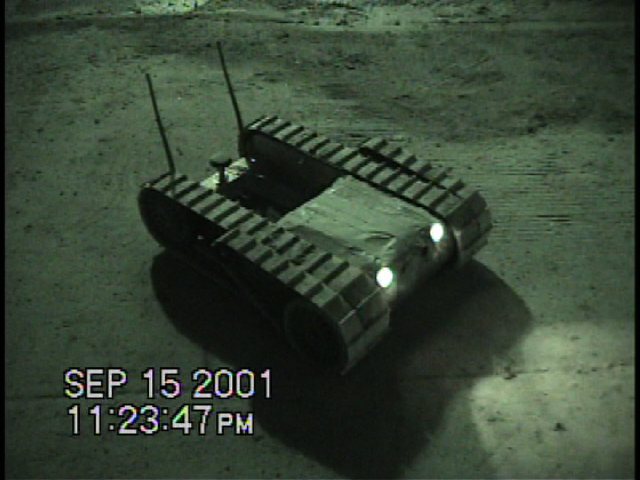
\includegraphics[width = \textwidth]{imagenes/Intro - PackBot.png}
        \caption{PackBot 510 \cite{AD_2021}}
        \label{fig: PackBot}
    \end{subfigure}
    \begin{subfigure}[c]{0.45\textwidth}
        \centering
        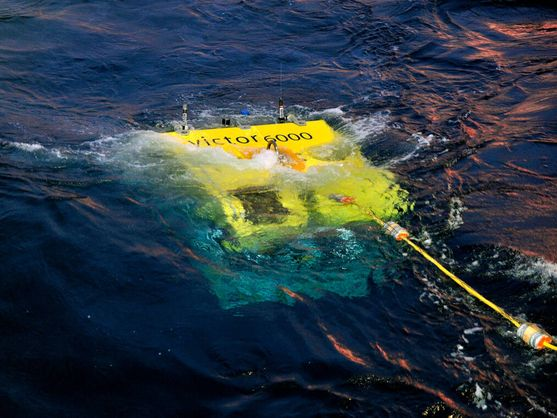
\includegraphics[width = \textwidth]{imagenes/Intro - Victor 6000.png}
        \caption{Victor 6000 \cite{Díaz_2023}}
        \label{fig:Victor 6000}
    \end{subfigure}
    \begin{subfigure}[c]{0.45\textwidth}
        \centering
        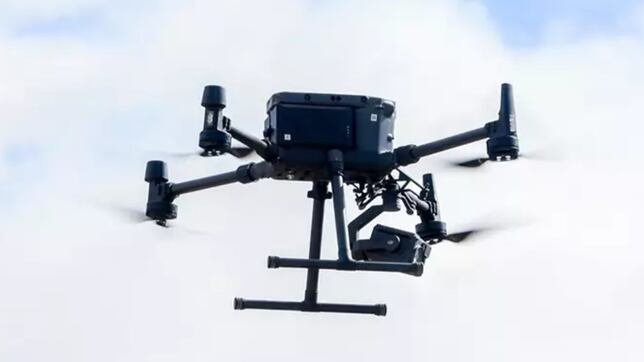
\includegraphics[width = \textwidth]{imagenes/Intro - Valencia.png}
        \caption{Matrice 300 RTX \cite{Cañas_2024}}
        \label{fig:Matrice 300 RTX}
    \end{subfigure}
    \caption{Robots de rescate.}
\end{figure}


La historia del robot Joker (Figura \ref{fig:Robot-Joker}) se hizo famosa recientemente a causa del fenómeno televisivo `Chernobyl' de HBO. Este robot alemán fue enviado a la Central Nuclear de Chernobyl para ayudar con las labores de limpieza de material radiactivo. Desafortunadamente, no salió como se esperaba y se perdió la comunicación con este. En un principio se pensó que se había quedado atascado entre los escombros pero se lo encontraron quemado. Actualmente `Joker' se encuentra abandonado en un depósito de chatarra en la zona de exclusión.

Una de las primeras intervenciones de un vehículo robótico en labores de búsqueda y rescate urbana, fue tras los atentados del 11 de Septiembre de 2001 contra las torres del World Trade Center de Nueva York. Uno de los robots utilizados fue el PackBot 510 (Figura \ref{fig: PackBot}), que tenía como misión buscar posibles víctimas bajo los escombros, además de evaluar la estructura y proporcionar imágenes de áreas inaccesibles por equipos de rescate humanos. El robot dispone de un sistema de oruga doble que le permite avanzar sobre cualquier terreno. Lleva incorporados un manipulador que permite levantar hasta 20 kg, además de sensores, cámaras y diferentes útiles intercambiables.

En Junio de 2023, tras la desaparición del submarino turístico que fue a visitar los restos del Titanic en el Océano Atlántico, Francia envió urgentemente a Víctor 6000 (Figura \ref{fig:Victor 6000}). Este robot está conectado a un buque mediante un cable de 8.000 metros que le suministra una potencia eléctrica de 20 kW. Es un dispositivo diseñado principalmente para llevar a cabo trabajos oceanográficos científicos, está equipado con un sistema de navegación de alto rendimiento, así como con un sistema de imagen óptica de alta resolución, tanto de fotografía como de vídeo, que permite tener una percepción visual del entorno.

Tras el incendio en un edificio en Valencia a finales de Febrero del 2024, el dron Matrice 300 RTX (Figura \ref{fig:Matrice 300 RTX}) trabajó junto a los bomberos en las labores de búsqueda de personas desaparecidas. Enviado por la Unidad Militar de Emergencias (UME) fue adquirido a finales del año 2022 por el Ministerio de Defensa. Es capaz de operar en misiones de rescate, con condiciones climatológicas adversas, alcanzando una velocidad máxima de 23 km/h, así como un alcance de hasta 15 km, y con una carga útil cercana a los 3 kg. Puede soportar rachas de viento de hasta 55 km/h, tiene equipada una cámara térmica radio-métrica, y un telémetro láser que permite medir distancias con precisión. No es la primera vez que la UME utiliza drones para misiones con estas características. El Mavic II, modelo similar al Matrice 300 RTX fue utilizado cuando entró en erupción el volcán en La Palma en 2021.


% Entrando en proyectos llevados a cabo en la Universidad de Málaga, encontramos el perro robot que acompaña a la policía local de Málaga (Figura \ref{fig: Perro UMA}). Diseñado por el Instituto de Tecnología e Ingeniería del Software (ITIS), en colaboración con la Unidad de Defensa y Seguridad de Telefónica y la pyme española Alysis, con la financiación de fondos Next Generation. Está dotado de cámaras que le permiten tomar fotografías y grabar vídeos, además de detectar si una persona está andado, tumbada o va en patinete. Actualmente, se encuentra en fase de prueba. En un principio estará acompañado y controlado manualmente por un policía local, pero se espera que en el futuro, gracias a la inteligencia artificial, gane autonomía y pueda patrullar en solitario.